\documentclass{beamer}
\usetheme{Frankfurt}

\usepackage{algpseudocodex}
\usepackage[pdf]{graphviz}
\usepackage{morewrites}

\usepackage{pgfpages}
\usepackage{awesomebox}
\usepackage{amsmath}
\usepackage{amssymb}
\usepackage{comment}
\usepackage{listings}
\usepackage{booktabs}

\newcommand{\itab}{Cormen et al. Introduction to Algorithms, Third Edition (3rd. ed.). The MIT Press.}

\newcommand{\seqa}[1]{$\lang #1 \rangle$}
\newcommand{\seqb}[2]{$#1 =\langle #2 \rangle$}
\setbeamertemplate{note page}{\pagecolor{yellow!5}\insertnote}\usepackage{palatino}

\AtBeginSection[]{
  \begin{frame}
  \vfill
  \centering
  \begin{beamercolorbox}[sep=8pt,center,shadow=true,rounded=true]{title}
    \usebeamerfont{title}\insertsectionhead\par%
  \end{beamercolorbox}
  \vfill
  \end{frame}
}

%\setbeameroption{show notes on second screen=right} % Both

\title{Design and Analysis of Algorithms}

\author{Rodrigo Bonif\'{a}cio}

\begin{document}
\begin{frame}
\titlepage
\end{frame}


%\input{chap01}
%\input{chap02}
%\input{chap03}
%\section{Graph Algorithms}

	\begin{frame}
          \frametitle{Graphs}

          Pervasive data structure in Computer Science---an abstract
          representation in use to describe different domains, including
          trasport systems, electrical circuits, human interactions (social networks),
          computer networks, and software dependencies. \pause This class aims to
          discuss two concerns:   

          \vskip+1.5em

          \begin{itemize}
            \item graph representation 
            \item graph algorithms 
          \end{itemize}
        \end{frame}

\begin{frame}
\frametitle{Definition}

A graph $G$ is a pair $(V, E)$ where $V$ is an arbitrary
set and $E$ is a subset of $V^{(2)}$\pause---the set of all pairs of
elements in $V$.  The elements of $V$ are the {\color{blue}vertices} of the
graph, while the elements of $E$ are the {\color{blue}edges}
of the graph. 


\pause \vskip+1.5em
\begin{block}{Different flavors of graphs}

\begin{itemize}
\item directed graphs $\times$ undirected graphs
\item weighted graphs $\times$ unweighted graphs
\item ciclic graphs $\times$ aciclic graphs
\item \ldots
\end{itemize}
\end{block}
\end{frame}

\begin{frame}
\frametitle{Graph representations}


\begin{itemize}
\item {\bf Adjacency-list:} compact representation recommended for
  {\color{blue}sparse graphs}  (where $|E|$ is smaller than 
  $|V|^{2}$). \pause 

\item {\bf Adjacency-matrix:} recommended for dense graphs or when we
  need to frequently search if an edge $(v_1, v_2)$ exists.   
\end{itemize}

\end{frame}

\begin{frame}
\frametitle{Samples (Fonte: Introduction to Algorithms)}
\centering{

\includegraphics[scale=0.5]{images/undirected01.png}

\pause 

\includegraphics[scale=0.5]{images/directed01.png}	
}

\end{frame}


\begin{frame}
  \frametitle{Graph Algorithms}

  \begin{itemize}
   \item Search: Breadth-first search and Depth-first Search
   \item Single-source shortest paths: Bellman-Ford and Dijkstra algorithms
   \item {\color{blue}All-pairs shortest paths}  
   \item {\color{blue}Minimum Spanning Trees}
  \end{itemize}
\end{frame}


\begin{frame}{All-pairs shortest paths}

  We are given a weighted, directed graph $G(V, E)$ with a
  weight function $w : E \rightarrow \mathbb{R}$, and our goal
  is to find, for {\color{blue}every} pair of vertices $u, v \in V$,
  the shortest path from $u$ to $v$.

  \pause

  \begin{block}{Note}
  \begin{itemize}
    \item Computing the single-source shortest paths to all
      vertices $v \in V$ is not efficient. \pause Here we will present a
      dynamic programming algorithm (Floyd-Warshal) that runs in $\Theta(V^3)$ 
  \end{itemize}
  \end{block}

\end{frame}

\begin{frame}{Floyd-Warshal algorithm}

  \begin{block}{Features}
    \begin{itemize}
     \item Represents the graph using an adjacency-matrix \pause (each cell $(u, v)$ in
       the matrx contains the weight of the edge $u \rightarrow v$). \pause

     \item Considers the intermediate vertices of a shortest path. If $p = \rangle v_1, v_2, \ldots, v_l \langle$,
       any vertex other than $v_1$ and $v_l$ are intermediate vertices. \pause

     \item Iterative: Under the assumption that $V = \{1, 2, \ldots, n\}$, considers the subsets $\{1, 2, \ldots, k\}$
       of vertices for some $k$. 
    \end{itemize}
  \end{block}
\end{frame}

\begin{frame}
  \centering{
    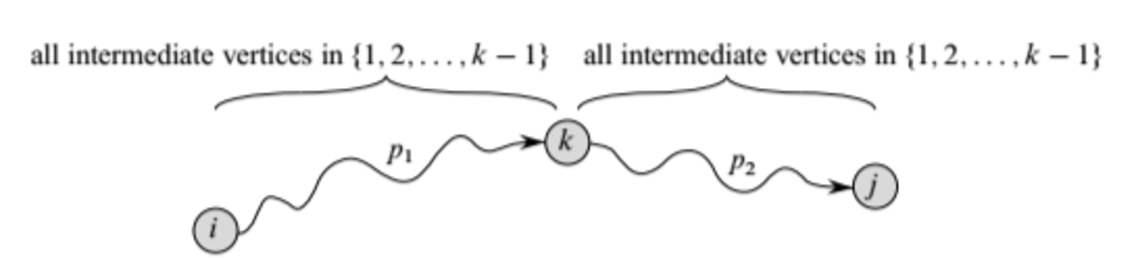
\includegraphics[scale=0.5]{images/fw}
   }
\end{frame}

\begin{frame}{Recursive Solution}

\[
d^{(k)}_{ij}= \left\{
\begin{array}{ll}
      w_{ij}                    & if\ k = 0\\ 
      min(d^{(k-1)}_{ij}, d^{(k-1)}_{ik}+d^{(k-1)}_{kj})  & if\ k \geq 1 \\   
\end{array} 
\right. 
\]

\pause

\begin{itemize}
  \item The matrix $D^{(n)}$ gives the final answer (considering $V = \{1, 2, \ldots, n\}$).
\end{itemize}
\end{frame}

\begin{frame}{Example}
    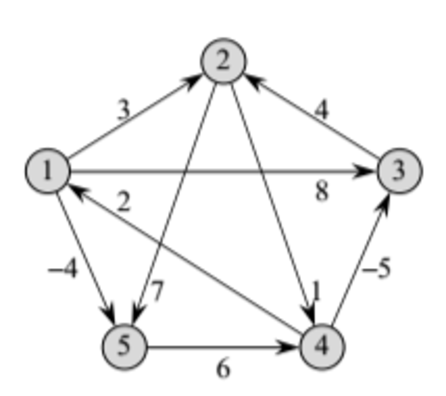
\includegraphics[scale=0.5]{images/graph-fw}
\end{frame}

\begin{frame}
  \centering{
    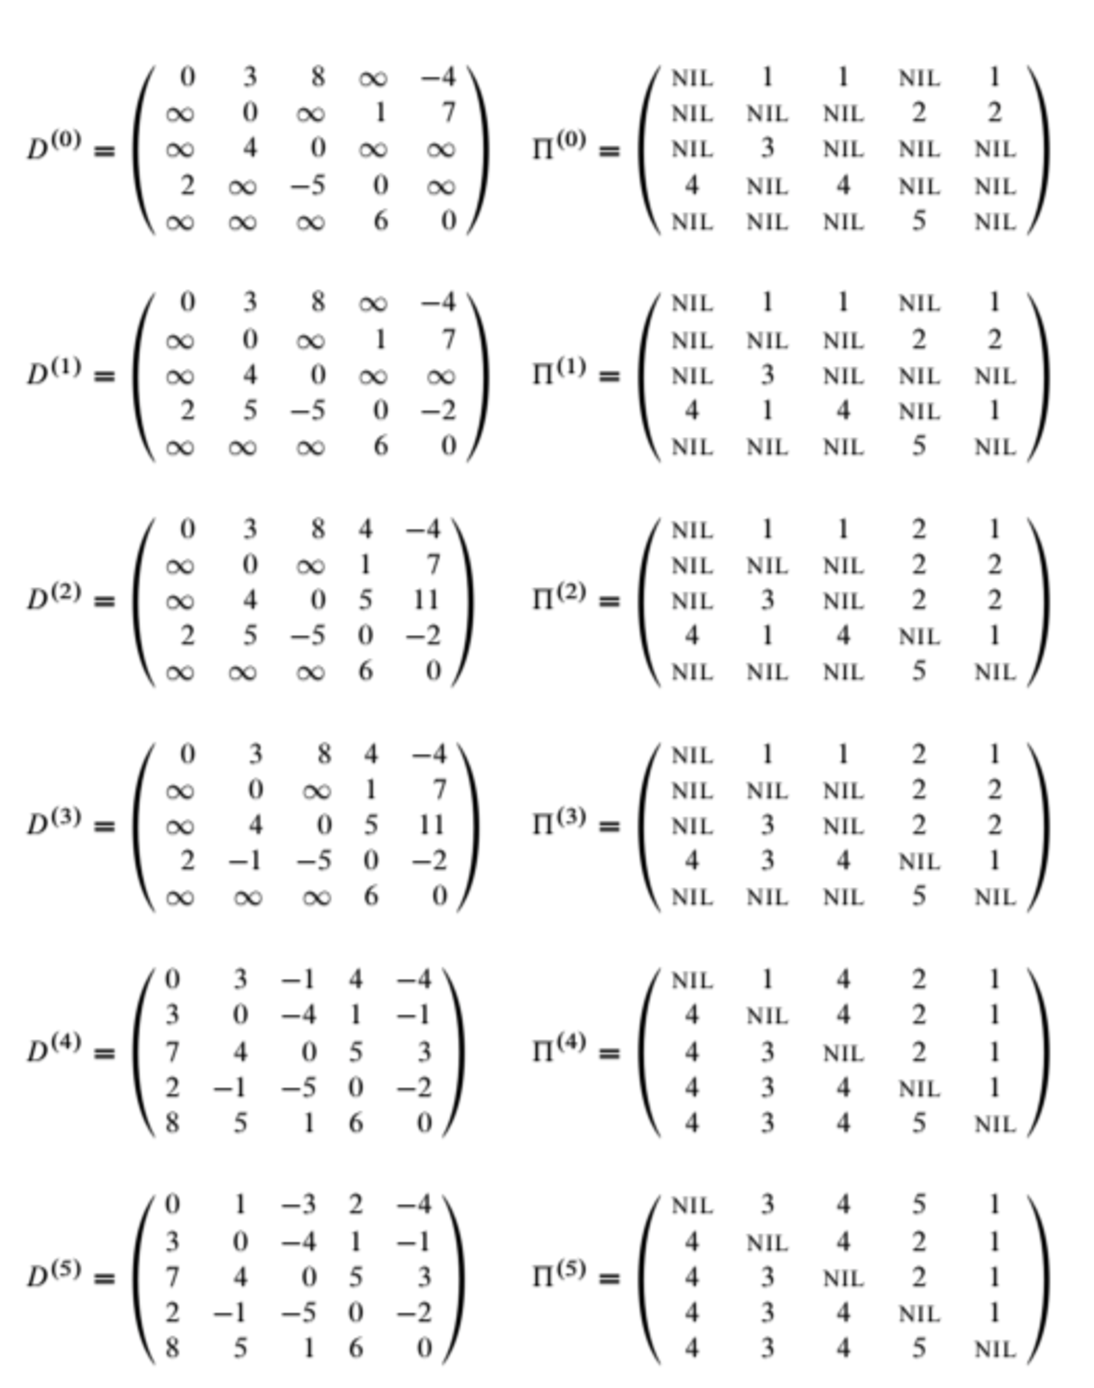
\includegraphics[scale=0.3]{images/fw-res}}
\end{frame}

\begin{frame}
  \begin{block}{Floyd-Warshall algorithm}
      \begin{algorithmic}
    \Procedure{Floyd-Warshall}{W}
     \State $n = W.rows$
     \State $D^{(0)} = W$
     \For{$k = 1 \ldots n$}
      \State $D^{(k)} = (d^{(k)}_{ij}) \text{ be a new n x n matrix}$
      \For{$i = 1 \ldots n$}
        \For{$j = 1 \ldots n$}
          \State $d^{(k)}_{ij} = min(d^{(k-1)}_{ij}, d^{(k-1)}_{ik}+d^{(k-1)}_{kj})$
        \EndFor
      \EndFor
     \EndFor
    \State {\bf return} $D^{(n)}$
    \EndProcedure 
  \end{algorithmic}
  \end{block}  
\end{frame}

\begin{frame}{Minimum Spanning Trees}

  Given a connected, weighted, and undirected graph $G = (V, E)$, we wish to
  find an acyclic subset $T \subseteq E$ that connects all of the vertices
  and whose {\color{blue}total} weight is minimized. \pause Since $T$ is acyclic and
  connects all of the vertices, it must form a (spanning) tree. 

  \pause \vskip+1.5em

  \centering{
    \includegraphics[scale=0.5]{images/st}
  }
\end{frame}


\begin{frame}

  The book presents an interesting description of the algortihms for
  Minimum Spanning Trees: a generic method for growing minimum spanning trees
  and two implementations of the algorithm (Kruskal's algorithm and Prim's algorithm).

  \pause \vskip+1.5em

  \begin{block}{Generic Method}
  \begin{algorithmic}
    \Procedure{Generic-MST}{G, w}
     \State $A = \emptyset$                 
     \While{$\text{A does not form a spanning tree}$}        
       \State $\text{find an edge (u, v) that is safe for A}$
       \State $A = A \cup \{(u, v)\}$
     \EndWhile
     \State {\bf return} $A$
    \EndProcedure
  \end{algorithmic}
  \end{block}

  \pause

  \begin{itemize}
    \item The challenge is to find out a {\color{blue}safe edge (u, v)}. 
  \end{itemize}
\end{frame}

\begin{frame}{Definitions}

  \begin{itemize}
   \item A {\color{blue}$cut(S, V-S)$} of an undirected graph $G = (V, E)$ is a partition of $V$. \pause 

   \item An {\color{blue}edge $(u, v) \in E$ crosses} a $cut(S, V-S)$ if one of its endpoints is in $S$ and
     the other is in $V-S$. \pause

   \item A {\color{blue}cut respects} a set A of edges if no edge in A crosses the cut. \pause
     
   \item An edge is a {\color{blue}light edge crossing} a cut if its weight is the minimum of any
     edge crossing the cut.  
  \end{itemize}
\end{frame}

\begin{frame}
  \begin{block}{Theorem}
    Given:
    \begin{itemize}
      \item $G = (V, E)$ is a connected, undirected graph
      \item $w : E \rightarrow \mathbb{R}$ is a weighted function.
      \item $A$ is a subset of $E$ (included in some minimum spanning subtree for $G$)
      \item $(S, V-S)$ is any cut of $G$ that respects $A$
      \item $(u, v)$ is a light edge crossing $(S, V-S)$
    \end{itemize}
    then, edge $(u, v)$ is safe for $A$. 
  \end{block}

  Both algorithm implementations relie on this theorem. 
\end{frame}

\begin{frame}
  In the Kruskal's algorithm, the set $A$ is a {\color{blue}forest}
  whose vertices are all those of the given graph. The safe edge
  added to $A$ is allways a lest-weight edge in the graph that
  connects two distinct trees in the forest. \pause The book
  shows an implementation that benefits from the Disjoint Set
  data structure, whose interface contains three operations:
  \texttt{makeSet}, \texttt{findSet}, and \texttt{union}. 
\end{frame}

\begin{frame}
  \begin{small}
  \begin{algorithmic}
    \Procedure{MST-Kruskal}{G, w}
    \For{$\text{each vertex v } \in G.V$}
      \State $makeSet(v)$
    \EndFor
    \State $lst = \text{sort the edges of G.E into nondecreasing order by weight w}$
    \For{$(u, v) \rightarrow lst$}
      \If{$findSet(u) \neq findSet(v)$}
       \State $A = A \cup \{(u, v)\}$
       \State $union(u, v)$
      \EndIf 
    \EndFor
    \State {\bf return} $A$  
    \EndProcedure
  \end{algorithmic}
  \end{small}
\end{frame}

\begin{frame}{TODO}

  Study and implement the Prim's algorithm for
  computing minimum spanning trees. 
 
\end{frame}

\section{Algorithms for Data Flow Analysis}


\begin{frame}
  \frametitle{Program Analysis\footnote{Pedro Costa and Luis Amaral contributed to these slides}}

  \begin{block}{Goal}
    Predict {\color{blue}safe} and {\color{blue}computable approximations} of the possible
    behaviours that arise at runtime when executing a program. \pause \\
    Usage Scenarios:
    \begin{itemize}
     \item program optimization
     \item program transformation
     \item program design metrics
     \item software security
    \end{itemize}
  \end{block}
\end{frame}

\begin{frame}
  \frametitle{The While Language}

  \begin{block}{Features}
    \begin{itemize}
     \item tiny (imperative) programming language
     \item integer and boolean expressions  
     \item conditionals and loops \pause
     \item every statement has a unique label  
    \end{itemize}
  \end{block}

\end{frame}

\begin{frame}
  \frametitle{An introduction to DataFlow Analysis}

  \begin{enumerate}
    \item The program is modeled as a (control-flow) graph: the nodes are the
  the elementary blocks (statements) and the edges describe how the
  control might pass from one statement to another.

    \item We define functions for every node, so that data flow information
      can be computed using pairs of \emph{Gen} and \emph{Kill} functions---considering the
      information produced in the previou(s) node(s). 
  \end{enumerate}

  \pause Computing a solution for a dataflow problem often
  requires multiple iteractions, where every new iteration
  provides a better approximation (monotone framework).
  The iteration continues until achieving a {\color{blue}fixpoint}.
  \pause $f(s) = s$
  
\end{frame}

\begin{frame}[fragile]
  \frametitle{Running Example}
  
  \begin{center}
  	\large Example 01: Factorial
  \end{center}
  
  \begin{columns}
    \column[t]{0.40\textwidth}
While language
    
\begin{verbatim}
y := x;           (1)
z := 1;           (2)
while(y > 1) do   (3)
  z := z * y;     (4) 
  y := y - 1;     (5) 
y := 0;           (6) 
\end{verbatim}
\column[t]{0.60\textwidth}
\pause Control Flow Graph
\digraph[scale=0.40]{cfg01}{
  node [fontname = "Handlee"];
  edge [fontname = "Handlee"];

  n1 [
    label = "y := x";
    shape = rect;
    xlabel="1";
  ];
  n2 [
    label = "z := 1";
    shape = rect;
    xlabel="2";
  ];
  n3 [
    label = "while y > 1";
    shape = diamond;
    xlabel="3";
  ];
  n4 [
    label = "z := z * y";
    shape = rect;
    xlabel="4";
  ];
  n5 [
    label = "y := y - 1";
    shape = rect;
    xlabel="5";
  ];
  n6 [
    label = "y := 0"; 
    shape = rect;
    xlabel="6";
  ]; 
  n1 -> n2;
  n2 -> n3;
  n3 -> n4[label = "yes"]
  n4 -> n5; 
  n5 -> n3; 
  n3 -> n6 [label = "no"];
  
  {
    rank=same;
    n3;n4;
  }
}

\end{columns}
\end{frame}


\subsection{Reaching Definitions}

\begin{frame}
  \begin{huge}
    Reaching Definitions
  \end{huge}
  \pause

  \vskip+1.5em
  
  \begin{itemize}
   \item Application in different areas, including {\color{blue}tainted analysis}.
   \item Allows the construction of \emph{def-use} and \emph{use-def} chains. These
     chains facilitate several transformations targeting program optimization. 
  \end{itemize}
\end{frame}

\begin{frame}
  \frametitle{Reaching Definitions Algorithm}

  \begin{block}{Informal definition}
   For every vertice \texttt{(from, to)} in the control flow,
   we check if \texttt{assignment(v, exp) := to} holds (\texttt{to} is
   an assignment).\pause If this is the case, we remove all definitions that
   assign a value to \texttt{v} ({\color{blue}Kill}) from the input set, and expose a new
   definition of \texttt{v} at statement \texttt{to} ({\color{blue}Gen}).
   If \texttt{to} is not a definition (an assignment), than we just propagate the
   sets of definitions that arrive at \texttt{to}.
  \end{block} 
\end{frame}

\begin{frame}{Equations for Reaching Definitions}
  \centering{
    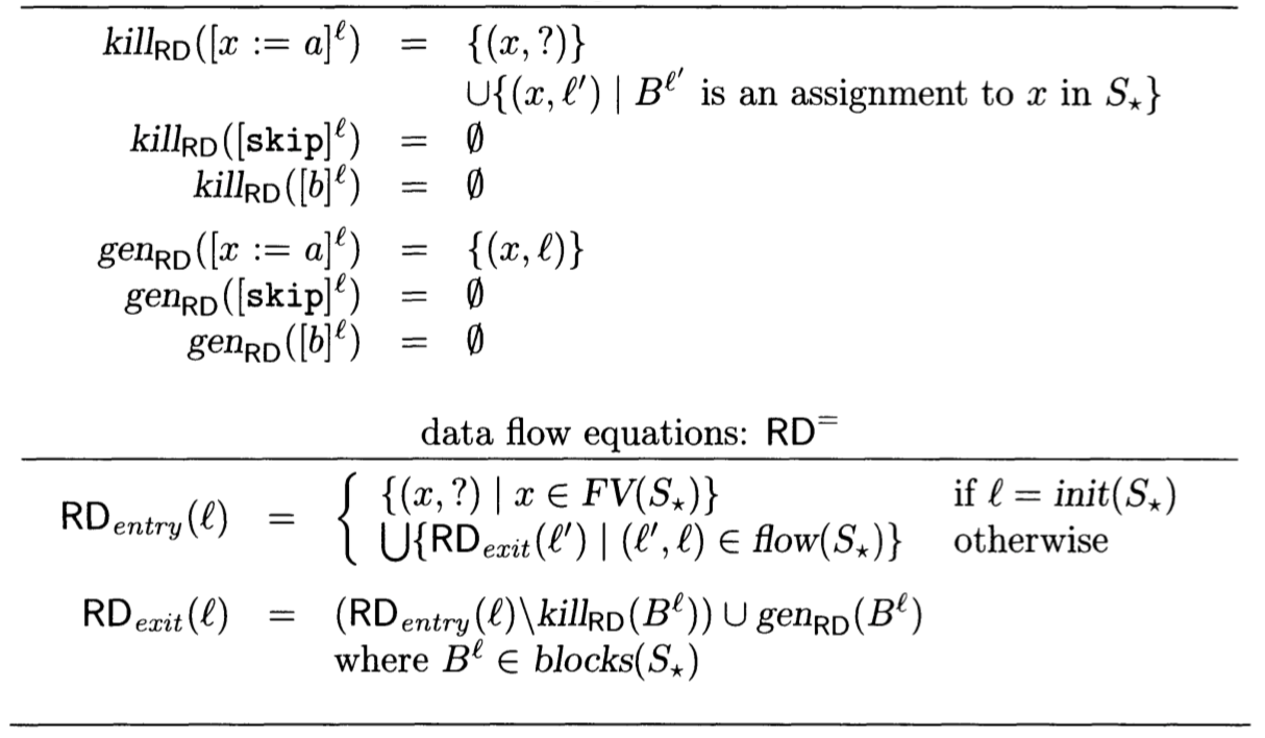
\includegraphics[scale=0.5]{images/rde}

    \scriptsize{Nielson et al. Principles of Program Analysis. Springer-Verlag. 2005}
  }
\end{frame}

\begin{frame}[fragile]
  \frametitle{Iterative Reaching Definitions Algorithm}

  \begin{block}{Equations}
    \begin{itemize}
    \item $Out(s) = Gen(s) \cup (In(s) - Kill(s))$  
    \item $In(s) = \bigcup_p Out(p), p \in pred(s), s \in stmts$
    \end{itemize}
  \end{block}

  \pause

\begin{block}{Iterative algorithm}
  \begin{algorithmic}
    \Procedure{ReachingDefinitions}{CFG}
     \State $Out[Start] = \{\}$ 
     \For{$s \leftarrow CFG.V$}
       \State{$Out[s] = \{ \}$}
     \EndFor
     \While{$\text{not fixed}$}
       \For{$s \leftarrow CFG.V$}
         \State{$\text{compute In[s]}$}
         \State{$\text{compute Out[s]}$}
       \EndFor
     \EndWhile
    \State {\bf return} $(In, Out)$
    \EndProcedure 
  \end{algorithmic}
\end{block}
\end{frame}



%%%%%%%%%%%%%%%%%%%%%%%%%%%%%%%%%%%%%%%%%%%%%%%%%%%%%%%%%
\begin{frame}[fragile, t]
 \frametitle{Iteration 1} 

\begin{center}
\begin{scriptsize}
\begin{minipage}{8cm}
    \begin{block}{Equations}
    \begin{itemize}
        \item $Out(s) = Gen(s) \cup (In(s) - Kill(s))$  
	    \item $In(s) = \bigcup_p Out(p), p \in pred(s), s \in stmts$
    \end{itemize}
    \end{block}
\end{minipage}
\end{scriptsize}
\end{center}

\begin{columns}[T]
\begin{column}[T]{.4\textwidth}
    \vspace{0pt}
    \digraph[scale=0.40]{cfg01}{
  node [fontname = "Handlee"];
  edge [fontname = "Handlee"];

  n1 [
    label = "y := x";
    shape = rect;
    xlabel="1";
  ];
  n2 [
    label = "z := 1";
    shape = rect;
    xlabel="2";
  ];
  n3 [
    label = "while y > 1";
    shape = diamond;
    xlabel="3";
  ];
  n4 [
    label = "z := z * y";
    shape = rect;
    xlabel="4";
  ];
  n5 [
    label = "y := y - 1";
    shape = rect;
    xlabel="5";
  ];
  n6 [
    label = "y := 0"; 
    shape = rect;
    xlabel="6";
  ]; 
  n1 -> n2;
  n2 -> n3;
  n3 -> n4[label = "yes"]
  n4 -> n5; 
  n5 -> n3; 
  n3 -> n6 [label = "no"];
  
  {
    rank=same;
    n3;n4;
  }
}

    \end{column}
    \begin{column}[T]{.6\textwidth}
\vspace{30pt}    
	\begin{scriptsize}
	   \begin{table}[]
\begin{tabular}{|l|l|l|}
\hline
n & IN{[}n{]} & OUT{[}n{]} \\ \hline
1  & \pause \{ \}            & \pause \{(y,1)\} \\ \hline
2  & \pause \{(y,1)\}        & \pause \{(y,1), (z,2)\} \\ \hline
3  & \pause \{(y,1), (z,2)\} & \pause \{(y,1), (z,2)\} \\ \hline
4  & \pause \{(y,1), (z,2)\} & \pause \{(y,1), (z,4)\} \\ \hline
5  & \pause \{(y,1), (z,4)\} & \pause \{(y,5), (z,4)\} \\ \hline
6  & \pause \{(y,1), (z,2)\} & \pause \{(y,6), (z,2)\} \\ \hline
\end{tabular}
\end{table}   
	\end{scriptsize}
	\end{column}
%\hfill
    
\end{columns}

\end{frame}



%%%%%%%%%%%%%%%%%%%%%%%%%%%%%%%%%%%%%%%%%%%%%%%%%%%%%%%%%
\begin{frame}[fragile, t]
	\frametitle{Iteration 2} 
	
	\vspace{-1cm}
	
	\begin{columns}[T]
		\begin{column}[T]{.4\textwidth}
	\begin{center}
		\begin{scriptsize}
			\begin{minipage}{8cm}
		%		\begin{block}{Equations}
					\begin{itemize}
						\item $Out(s) = Gen(s) \cup (In(s) - Kill(s))$  
						\item $In(s) = \bigcup_p Out(p), p \in pred(s), s \in stmts$
					\end{itemize}
		%		\end{block}
			\end{minipage}
		\end{scriptsize}
	\end{center}
\end{column}
\begin{column}[T]{.6\textwidth}
	\begin{tiny}
		   \begin{table}[]
		\begin{tabular}{|l|l|l|}
			\hline			
			\multicolumn{3}{|c|}{Iteration 1}\\
			\hline
			n & IN{[}n{]} & OUT{[}n{]} \\ \hline
			1  & \{ \}            & \{(y,1)\} \\ \hline
			2  & \{(y,1)\}        & \{(y,1), (z,2)\} \\ \hline
			3  & \{(y,1), (z,2)\} & \{(y,1), (z,2)\} \\ \hline
			4  & \{(y,1), (z,2)\} & \{(y,1), (z,4)\} \\ \hline
			5  & \{(y,1), (z,4)\} & \{(y,5), (z,4)\} \\ \hline
			6  & \{(y,1), (z,2)\} & \{(y,6), (z,2)\} \\ \hline
		\end{tabular}
	\end{table}   
\end{tiny}
\end{column}
	\end{columns}
	
	\begin{columns}[T]
		\begin{column}[T]{.3\textwidth}
			\vspace{0pt}
			\digraph[scale=0.40]{cfg01}{
  node [fontname = "Handlee"];
  edge [fontname = "Handlee"];

  n1 [
    label = "y := x";
    shape = rect;
    xlabel="1";
  ];
  n2 [
    label = "z := 1";
    shape = rect;
    xlabel="2";
  ];
  n3 [
    label = "while y > 1";
    shape = diamond;
    xlabel="3";
  ];
  n4 [
    label = "z := z * y";
    shape = rect;
    xlabel="4";
  ];
  n5 [
    label = "y := y - 1";
    shape = rect;
    xlabel="5";
  ];
  n6 [
    label = "y := 0"; 
    shape = rect;
    xlabel="6";
  ]; 
  n1 -> n2;
  n2 -> n3;
  n3 -> n4[label = "yes"]
  n4 -> n5; 
  n5 -> n3; 
  n3 -> n6 [label = "no"];
  
  {
    rank=same;
    n3;n4;
  }
}

		\end{column}
		\begin{column}[T]{.7\textwidth}
			\vspace{0pt}    
			\begin{scriptsize}
				\begin{table}[]
					\begin{tabular}{|l|l|l|}
						\hline
						n  & IN{[}n{]} & OUT{[}n{]} \\ \hline
						1  & \pause \{ \}                          & \pause \{(y,1)\} \\ \hline
						2  & \pause \{(y,1)\}                      & \pause \{(y,1), (z,2)\} \\ \hline
						3  & \pause \{(y,1), (z,2), (y,5), (z,4)\} & \pause \{(y,1), (z,2), (y,5), (z,4)\} \\ \hline
						4  & \pause \{(y,1), (z,2), (y,5), (z,4)\} & \pause \{(y,1), (y,5), (z,4)\} \\ \hline
						5  & \pause \{(y,1), (y,5), (z,4)\}        & \pause \{(y,5), (z,4)\} \\ \hline
						6  & \pause \{(y,1), (z,2), (y,5), (z,4)\} & \pause \{(y,6), (z,2), (z,4)\} \\ \hline
					\end{tabular}
				\end{table}   
			\end{scriptsize}
		\end{column}
		%\hfill
		
	\end{columns}
	
\end{frame}



%%%%%%%%%%%%%%%%%%%%%%%%%%%%%%%%%%%%%%%%%%%%%%%%%%%%%%%%%
\begin{frame}[fragile, t]
	\frametitle{Iteration 3} 
	
	\vspace{-1cm}
	
	\begin{columns}[T]
		\begin{column}[T]{.4\textwidth}
			\begin{center}
				\begin{tiny}
					\begin{minipage}{8cm}
		%				\begin{block}{Equations}
							\begin{itemize}
								\item $Out(s) = Gen(s) \cup (In(s) - Kill(s))$  
								\item $In(s) = \bigcup_p Out(p), p \in pred(s), s \in stmts$
							\end{itemize}
		%				\end{block}
					\end{minipage}
				\end{tiny}
			\end{center}
		\end{column}
		\begin{column}[T]{.6\textwidth}
			\begin{tiny}
				\begin{table}[]
					\begin{tabular}{|l|l|l|}
						\hline			
						\multicolumn{3}{|c|}{Iteration 2}\\
						\hline
						n  & IN{[}n{]} & OUT{[}n{]} \\ \hline
						1  & \{ \}                          & \{(y,1)\} \\ \hline
						2  & \{(y,1)\}                      & \{(y,1), (z,2)\} \\ \hline
						3  & \{(y,1), (z,2), (y,5), (z,4)\} & \{(y,1), (z,2), (y,5), (z,4)\} \\ \hline
						4  & \{(y,1), (z,2), (y,5), (z,4)\} & \{(y,1), (y,5), (z,4)\} \\ \hline
						5  & \{(y,1), (y,5), (z,4)\}        & \{(y,5), (z,4)\} \\ \hline
						6  & \{(y,1), (z,2), (y,5), (z,4)\} & \{(y,6), (z,2), (z,4)\} \\ \hline
					\end{tabular}
				\end{table}   
			\end{tiny}
		\end{column}
	\end{columns}
	
	\begin{columns}[T]
		\begin{column}[T]{.3\textwidth}
			\vspace{0pt}
			\digraph[scale=0.40]{cfg01}{
  node [fontname = "Handlee"];
  edge [fontname = "Handlee"];

  n1 [
    label = "y := x";
    shape = rect;
    xlabel="1";
  ];
  n2 [
    label = "z := 1";
    shape = rect;
    xlabel="2";
  ];
  n3 [
    label = "while y > 1";
    shape = diamond;
    xlabel="3";
  ];
  n4 [
    label = "z := z * y";
    shape = rect;
    xlabel="4";
  ];
  n5 [
    label = "y := y - 1";
    shape = rect;
    xlabel="5";
  ];
  n6 [
    label = "y := 0"; 
    shape = rect;
    xlabel="6";
  ]; 
  n1 -> n2;
  n2 -> n3;
  n3 -> n4[label = "yes"]
  n4 -> n5; 
  n5 -> n3; 
  n3 -> n6 [label = "no"];
  
  {
    rank=same;
    n3;n4;
  }
}

		\end{column}
		\begin{column}[T]{.7\textwidth}
			\vspace{0pt}    
			\begin{scriptsize}
				\begin{table}[]
					\begin{tabular}{|l|l|l|}
						\hline
						n  & IN{[}n{]} & OUT{[}n{]} \\ \hline
						1  & \pause \{ \}                          & \pause \{(y,1)\} \\ \hline
						2  & \pause \{(y,1)\}                      & \pause \{(y,1), (z,2)\} \\ \hline
						3  & \pause \{(y,1), (z,2), (y,5), (z,4)\} & \pause \{(y,1), (z,2), (y,5), (z,4)\} \\ \hline
						4  & \pause \{(y,1), (z,2), (y,5), (z,4)\} & \pause \{(y,1), (y,5), (z,4)\} \\ \hline
						5  & \pause \{(y,1), (y,5), (z,4)\}        & \pause \{(y,5), (z,4)\} \\ \hline
						6  & \pause \{(y,1), (z,2), (y,5), (z,4)\} & \pause \{(y,6), (z,2), (z,4)\} \\ \hline
					\end{tabular}
				\end{table}   
			\end{scriptsize}
		\end{column}
		%\hfill
		
	\end{columns}
	
\end{frame}   



%%%%%%%%%%%%%%%%%%%%%%%%%%%%%%%%%%%%%%%%%%%%%%%%%%%%%%%%%
\begin{frame}[fragile, t]
	\frametitle{Iteration 3 (fixed point)} 
	
	\vspace{-1cm}
	
	\begin{columns}[T]
		\begin{column}[T]{.4\textwidth}
			\begin{center}
				\begin{tiny}
					\begin{minipage}{8cm}
		%				\begin{block}{Equations}
							\begin{itemize}
								\item $Out(s) = Gen(s) \cup (In(s) - Kill(s))$  
								\item $In(s) = \bigcup_p Out(p), p \in pred(s), s \in stmts$
							\end{itemize}
		%				\end{block}
					\end{minipage}
				\end{tiny}
			\end{center}
		\end{column}
		\begin{column}[T]{.6\textwidth}
			\begin{tiny}
				\begin{table}[]
					\begin{tabular}{|l|l|l|}
						\hline			
						\multicolumn{3}{|c|}{Iteration 2}\\
						\hline
						n  & IN{[}n{]} & OUT{[}n{]} \\ \hline
						1  & \{ \}                          & \{(y,1)\} \\ \hline
						2  & \{(y,1)\}                      & \{(y,1), (z,2)\} \\ \hline
						3  & \{(y,1), (z,2), (y,5), (z,4)\} & \{(y,1), (z,2), (y,5), (z,4)\} \\ \hline
						4  & \{(y,1), (z,2), (y,5), (z,4)\} & \{(y,1), (y,5), (z,4)\} \\ \hline
						5  & \{(y,1), (y,5), (z,4)\}        & \{(y,5), (z,4)\} \\ \hline
						6  & \{(y,1), (z,2), (y,5), (z,4)\} & \{(y,6), (z,2), (z,4)\} \\ \hline
					\end{tabular}
				\end{table}   
			\end{tiny}
		\end{column}
	\end{columns}
	
	\begin{columns}[T]
		\begin{column}[T]{.3\textwidth}
			\vspace{0pt}
			\digraph[scale=0.40]{cfg01}{
  node [fontname = "Handlee"];
  edge [fontname = "Handlee"];

  n1 [
    label = "y := x";
    shape = rect;
    xlabel="1";
  ];
  n2 [
    label = "z := 1";
    shape = rect;
    xlabel="2";
  ];
  n3 [
    label = "while y > 1";
    shape = diamond;
    xlabel="3";
  ];
  n4 [
    label = "z := z * y";
    shape = rect;
    xlabel="4";
  ];
  n5 [
    label = "y := y - 1";
    shape = rect;
    xlabel="5";
  ];
  n6 [
    label = "y := 0"; 
    shape = rect;
    xlabel="6";
  ]; 
  n1 -> n2;
  n2 -> n3;
  n3 -> n4[label = "yes"]
  n4 -> n5; 
  n5 -> n3; 
  n3 -> n6 [label = "no"];
  
  {
    rank=same;
    n3;n4;
  }
}

		\end{column}
		\begin{column}[T]{.7\textwidth}
			\vspace{0pt}    
			\begin{scriptsize}
				\begin{table}[]
					\begin{tabular}{|l|l|l|}
						\hline
						n  & IN{[}n{]} & OUT{[}n{]} \\ \hline
						1  & \{ \}                          & \{(y,1)\} \\ \hline
						2  & \{(y,1)\}                      & \{(y,1), (z,2)\} \\ \hline
						3  & \{(y,1), (z,2), (y,5), (z,4)\} & \{(y,1), (z,2), (y,5), (z,4)\} \\ \hline
						4  & \{(y,1), (z,2), (y,5), (z,4)\} & \{(y,1), (y,5), (z,4)\} \\ \hline
						5  & \{(y,1), (y,5), (z,4)\}        & \{(y,5), (z,4)\} \\ \hline
						6  & \{(y,1), (z,2), (y,5), (z,4)\} & \{(y,6), (z,2), (z,4)\} \\ \hline
					\end{tabular}
				\end{table}   
			\end{scriptsize}
		\end{column}
		%\hfill
		
	\end{columns}
	
\end{frame}   


\begin{frame}
  \begin{huge}
    Very busy expressions
  \end{huge}
  
  \pause
  
  \vskip+1.5em
  
  \begin{itemize}
  	\item An expression is very busy at the exit from a label if, no matter what path
  	is taken from the label, the expression must always be used before any of the
  	variables occurring in it are redefined.~\cite{ppa-book}. \pause The goal is to
        eliminate redundant computations of expressions. \pause 
  \end{itemize}
  
\end{frame}



\begin{frame}
	Questions:
	
	\begin{itemize}
		\item what is the ``shape'' of the data types? \pause
		\item what {\color{blue}meet} operator is the best fit for our problem?
		\item what {\color{blue}CFG} should we use (forward or backward)?   
		\item how would you define the {\color{blue}Gen} and {\color{blue}Kill} functions?   
	\end{itemize}
	
\end{frame}

\begin{frame}{Equations for Very Busy Expressions}
    \centering{
    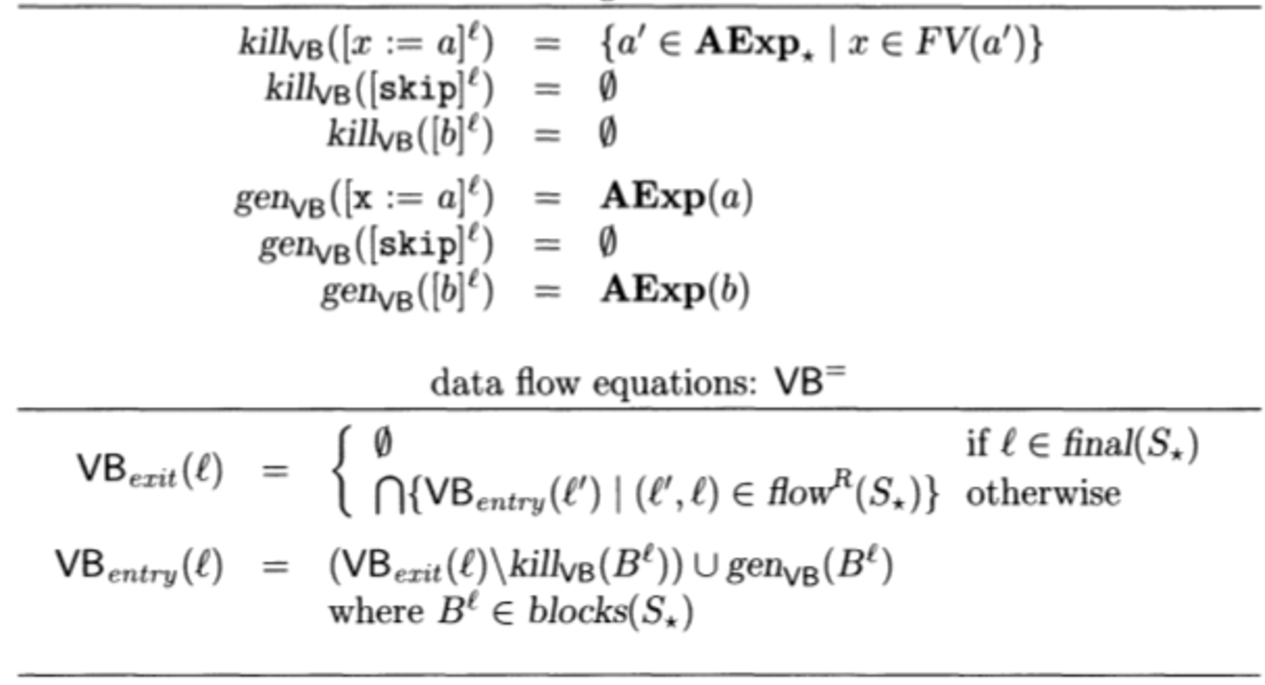
\includegraphics[scale=0.5]{images/vbe}
    \scriptsize{Nielson et al. Principles of Program Analysis. Springer-Verlag. 2005}}
\end{frame}

\begin{frame}[fragile]
	\frametitle{Very Busy Expressions Algorithm}
	
	\begin{block}{Equations}
		\begin{itemize}
			\item $Out(s) = \bigcap_p In(p), p \in successors(s), s \in stmts$
			\item $In(s) = Gen(s) \cup (Out(s) - Kill(s))$  
		\end{itemize}
	\end{block}
	
	\pause
	
	\begin{block}{Iterative algorithm}
          \begin{algorithmic}
            \Procedure{VeryBusyExpression}{CFG}
              \State $U = AExp_* \text{//se of non trivial expressions}$   
              \State $In[End] = \{\}$ 
              \For{$s \leftarrow CFG.V$}
                \State{$In[s] = U$}
              \EndFor
              \While{$\text{not fixed}$}
                 \For{$s \leftarrow CFG.V$}
                    \State{$\text{compute Out[s]}$}
                    \State{$\text{compute In[s]}$}
                  \EndFor
              \EndWhile
              \State {\bf return} $(In, Out)$
          \EndProcedure 
          \end{algorithmic}
	\end{block}
\end{frame}


\begin{frame}[fragile]
    \begin{columns}
    \column[t]{0.5\textwidth}
    Control Flow Graph
    \digraph[scale=0.35]{VbWhile} {
node [fontname = "Handlee"];
edge [fontname = "Handlee"];

start [
 label = "start";
 shape = ellipse; 
];

n1 [
 label = "if(a != b)";
 shape = diamond;
 xlabel="1";
];

n2 [
 label = "x := b - a";
 shape = rect;
 xlabel="2";
];

n3 [
 label = "y := a - b";
 shape = rect;
 xlabel="3";
];

n4 [
 label = "y := b - a";
 shape = rect;
 xlabel="4";
];

n5 [
 label = "a := 0";
 shape = rect;
 xlabel="5";
];

n6 [
 label = "x := a - b";
 shape = rect;
 xlabel="6";
];

end [
 label = "End";
 shape = ellipse; 
];

start -> n1;
n1 -> n2[label = "yes"];
n1 -> n4[label = "no"];
n2 -> n3;
n3 -> end;
n4 -> n5 -> n6;
n6 -> end;


{
rank=same;
n2;n4;
}

{
rank=same;
n3;n6;
}

}
    
    
    \column[t]{0.5\textwidth}
Example 04 (WHILE language)
    
\begin{verbatim}
if(a != b) then  (1)
  x := b - a;    (2)
  y := a - b;    (3)
else    
  y := b - a;    (4) 
  a = 0;         (5) 
  x = a- b;      (6) 
\end{verbatim}
\end{columns}
\end{frame}



\begin{frame}[fragile, t]
	\frametitle{Iteration 0} 
	
	\begin{center}
		\begin{scriptsize}
			\begin{minipage}{8cm}
				\begin{block}{Equations}
					\begin{itemize}
						\item $Out(s) = \bigcap_p In(p), p \in successors(s), s \in stmts$
						\item $In(s) = Gen(s) \cup (Out(s) - Kill(s))$  
					\end{itemize}
				\end{block}
			\end{minipage}
		\end{scriptsize}
	\end{center}
	
	\begin{columns}[T]
		\begin{column}[T]{.5\textwidth}
			\vspace{0pt}
			\digraph[scale=0.35]{VbWhile} {
node [fontname = "Handlee"];
edge [fontname = "Handlee"];

start [
 label = "start";
 shape = ellipse; 
];

n1 [
 label = "if(a != b)";
 shape = diamond;
 xlabel="1";
];

n2 [
 label = "x := b - a";
 shape = rect;
 xlabel="2";
];

n3 [
 label = "y := a - b";
 shape = rect;
 xlabel="3";
];

n4 [
 label = "y := b - a";
 shape = rect;
 xlabel="4";
];

n5 [
 label = "a := 0";
 shape = rect;
 xlabel="5";
];

n6 [
 label = "x := a - b";
 shape = rect;
 xlabel="6";
];

end [
 label = "End";
 shape = ellipse; 
];

start -> n1;
n1 -> n2[label = "yes"];
n1 -> n4[label = "no"];
n2 -> n3;
n3 -> end;
n4 -> n5 -> n6;
n6 -> end;


{
rank=same;
n2;n4;
}

{
rank=same;
n3;n6;
}

}
		\end{column}
		\begin{column}[T]{.5\textwidth}
			\vspace{30pt}    
			\begin{scriptsize}
				\begin{table}[]
					\begin{tabular}{|l|l|l|}
						\hline
						n & IN{[}n{]} & OUT{[}n{]} \\ \hline
						6  & \{ \} & \{ a - b, b - a \}  \\ \hline
						5  & \{ \} & \{ a - b, b - a \}  \\ \hline
						4  & \{ \} & \{ a - b, b - a \}  \\ \hline
						3  & \{ \} & \{ a - b, b - a \}  \\ \hline
						2  & \{ \} & \{ a - b, b - a \} \\ \hline
						1  & \{ \} & \{ \} \\ \hline
					\end{tabular}
				\end{table}   
			\end{scriptsize}
		\end{column}
		%\hfill
		
	\end{columns}
	
\end{frame}



\begin{frame}[fragile, t]
 \frametitle{Iteration 1} 

\begin{center}
\begin{scriptsize}
\begin{minipage}{8cm}
    \begin{block}{Equations}
    \begin{itemize}
        \item $Out(s) = \bigcap_p In(p), p \in successors(s), s \in stmts$
	    \item $In(s) = Gen(s) \cup (Out(s) - Kill(s))$  
    \end{itemize}
    \end{block}
\end{minipage}
\end{scriptsize}
\end{center}

\begin{columns}[T]
\begin{column}[T]{.4\textwidth}
    \vspace{0pt}
    \digraph[scale=0.35]{VbWhile} {
node [fontname = "Handlee"];
edge [fontname = "Handlee"];

start [
 label = "start";
 shape = ellipse; 
];

n1 [
 label = "if(a != b)";
 shape = diamond;
 xlabel="1";
];

n2 [
 label = "x := b - a";
 shape = rect;
 xlabel="2";
];

n3 [
 label = "y := a - b";
 shape = rect;
 xlabel="3";
];

n4 [
 label = "y := b - a";
 shape = rect;
 xlabel="4";
];

n5 [
 label = "a := 0";
 shape = rect;
 xlabel="5";
];

n6 [
 label = "x := a - b";
 shape = rect;
 xlabel="6";
];

end [
 label = "End";
 shape = ellipse; 
];

start -> n1;
n1 -> n2[label = "yes"];
n1 -> n4[label = "no"];
n2 -> n3;
n3 -> end;
n4 -> n5 -> n6;
n6 -> end;


{
rank=same;
n2;n4;
}

{
rank=same;
n3;n6;
}

}
    \end{column}
    \begin{column}[T]{.6\textwidth}
\vspace{30pt}    
	\begin{scriptsize}
	   \begin{table}[]
\begin{tabular}{|l|l|l|}
\hline
n & IN{[}n{]} & OUT{[}n{]} \\ \hline
6  & \{ a - b \} & \{ \} \pause \\ \hline
5  & \{ \} & \{a - b\} \pause \\ \hline
4  & \{ b - a \} & \{ \} \pause \\ \hline
3  & \{ a - b \} & \{ \} \pause \\ \hline
2  & \{ a - b, b - a \} & \{ a - b \}\pause \\ \hline
1  & \{ b - a \} & \{  \}\pause \\ \hline
\end{tabular}
\end{table}   
	\end{scriptsize}
	\end{column}
%\hfill
    
\end{columns}

\end{frame}






















%% \begin{frame}[fragile]
%%     \begin{columns}
%%     \column[t]{0.5\textwidth}
%% Example 05 (Jimple (simplified))
    
%% \begin{verbatim}
%%   if(a = b) goto label1 (1)
%%   x := b - a;           (2)
%%   y := a - b;           (3)
%%   goto label2           (7)
%% label 1:
%%   y := b - a;           (4) 
%%   a = 0;                (5) 
%%   x = a- b;             (6)
%% label 2:
%%   return;               (8)
%% \end{verbatim}

%% \column[t]{0.5\textwidth}
%% Control Flow Graph
%% \digraph[scale=0.35]{VbJimple} {
node [fontname = "Handlee"];
edge [fontname = "Handlee"];

start [
 label = "start";
 shape = ellipse; 
];

n1 [
 label = "if a == b goto label1";
 shape = diamond;
 xlabel="1";
];

n2 [
 label = "x = b - a";
 shape = rect;
 xlabel="2";
];

n3 [
 label = "y = a - b";
 shape = rect;
 xlabel="3";
];

n4 [
 label = "y = b - a";
 shape = rect;
 xlabel="4";
];

n5 [
 label = "a = 0";
 shape = rect;
 xlabel="5";
];

n6 [
 label = "x = a - b";
 shape = rect;
 xlabel="6";
];

n7 [
 label = "goto label2";
 shape = rect;
 xlabel="7";
];

n8 [
 label = "return";
 shape = rect;
 xlabel="8";
];

end [
 label = "End";
 shape = ellipse; 
];

start -> n1;
n1 -> n2[label = "true"];
n1 -> n4[label = "false"];
n2 -> n3 -> n7;
n4 -> n5 -> n6;
n6 -> n8;
n7 -> n8;
n8 -> end;

}
%% \end{columns}
  
%% \end{frame}




%% \begin{frame}[fragile, t]
%%  \frametitle{Iteration 1} 

%% \begin{center}
%% \begin{scriptsize}
%% \begin{minipage}{8cm}
%%     \begin{block}{Equations}
%%     \begin{itemize}
%%         \item $Out(s) = \bigcap_p In(p), p \in successors(s), s \in stmts$
%% 	    \item $In(s) = Gen(s) \cup (Out(s) - Kill(s))$  
%%     \end{itemize}
%%     \end{block}
%% \end{minipage}
%% \end{scriptsize}
%% \end{center}

%% \begin{columns}[T]
%% \begin{column}[T]{.5\textwidth}
%%     \vspace{0pt}
%%     \digraph[scale=0.35]{VbJimple} {
node [fontname = "Handlee"];
edge [fontname = "Handlee"];

start [
 label = "start";
 shape = ellipse; 
];

n1 [
 label = "if a == b goto label1";
 shape = diamond;
 xlabel="1";
];

n2 [
 label = "x = b - a";
 shape = rect;
 xlabel="2";
];

n3 [
 label = "y = a - b";
 shape = rect;
 xlabel="3";
];

n4 [
 label = "y = b - a";
 shape = rect;
 xlabel="4";
];

n5 [
 label = "a = 0";
 shape = rect;
 xlabel="5";
];

n6 [
 label = "x = a - b";
 shape = rect;
 xlabel="6";
];

n7 [
 label = "goto label2";
 shape = rect;
 xlabel="7";
];

n8 [
 label = "return";
 shape = rect;
 xlabel="8";
];

end [
 label = "End";
 shape = ellipse; 
];

start -> n1;
n1 -> n2[label = "true"];
n1 -> n4[label = "false"];
n2 -> n3 -> n7;
n4 -> n5 -> n6;
n6 -> n8;
n7 -> n8;
n8 -> end;

}
%%     \end{column}
%%     \begin{column}[T]{.5\textwidth}
%% \vspace{30pt}    
%% 	\begin{scriptsize}
%% 	   \begin{table}[]
%% \begin{tabular}{|l|l|l|}
%% \hline
%% n & IN{[}n{]} & OUT{[}n{]} \\ \hline
%% 8  & \{ \} & \{ \} \pause \\ \hline
%% 7  & \{ \} & \{ \} \pause \\ \hline
%% 6  & \{ \} & \{ \} \pause \\ \hline
%% 5  & \{ \} & \{ \} \pause \\ \hline
%% 4  & \{ \} & \{ \} \pause \\ \hline
%% 3  & \{ \} & \{ \} \pause \\ \hline
%% 2  & \{ \} & \{ \} \pause \\ \hline
%% 1  & \{ \} & \{ \} \pause \\ \hline
%% \end{tabular}
%% \end{table}   
%% 	\end{scriptsize}
%% 	\end{column}
%% %\hfill
    
%% \end{columns}

%% \end{frame}

\section{Complexity Theory}

\begin{frame}
  Most of the algorithms we explored in this course
  have been \emph{polynomial-time algorithms} (aka easy problems)\pause---that is,
  their worst-case running time is $\mathcal{O}(n^k)$.

    \begin{itemize}
     \item There are (hard) problems that can be solved, but not in time $\mathcal{O}(n^k)$ (for any constant $k$). 
     \item There are problems that cannot be solved by any computer (e.g., {\color{blue}The Halting Problem}), no metter
       how much computing time is available. 
    \end{itemize}
\end{frame}

\begin{frame}{P class of problems}
  \begin{itemize}
    \item The class P comprehends problems that we can solve in
    polynomial time ($\mathcal{O}(n^k)$).
  \end{itemize}    
\end{frame}


\begin{frame}{NP class of problems}
  \begin{itemize}
  \item The class NP comprehends problems that are verifiable
    in polynomial time. \pause That is, we are able to {\color{blue}check
    in polynomial time} the correctness of an answer for a
    specific instance of the problem.
  \item Example: we can check in polynomial time if an assignment to boolean variables
    satisfies a 3-CNF formula. However, we cannot answer if a 3-CNF formula is
    satisfiable in polynomial time. 
  \end{itemize}
\end{frame}  

\begin{frame}
  \begin{huge}
    Any problem in P is also in NP ($P \subseteq NP$).
  \end{huge} \pause

  \vskip+1.5em

  
  \begin{itemize}
   \item Open question: $P \subsetneq NP$
   \item NPC (NP-complete) is the set of problems that are in NP and
     are as ``hard'' as any problem in NP. \pause If an NPC problem could
     be solved in polynomial time, then all problems in NP has a polynomial
     time algorithm. \pause Most theoretical computer scientists believe that NPC
     problems are intractable.
  \end{itemize}
\end{frame}


\end{document}





